\chapter{Introduction}

\section{Motivation}
Carbonaceous nanoparticles, such as Carbon Black (CB) and soot, are widely encountered in nature and engineering. Every year, nearly 9.5 megatons of soot (black carbon) is emitted into the atmosphere from anthropogenic activities and natrual sources such as wildfires and volcanoes~\citep{myhre2014anthropogenic}. The wide light absorption range of soot reduces the albedo of snow-covered area and alters the radiative forcing balance in the atmosphere making soot the third strongest contributor to climate change after methane and carbon dioxide~\citep{myhre2014anthropogenic}. Also, exposure to combustion-generated soot could promote respiratory and cardiovascular disease~\citep{world2013health}. So, strict regulations are targeting combustion engines to limit environmental and health risks from soot formation~\citep{integrated2019}. Accurate and affordable models are essential for the prediction of soot composition and morphology in combustion devices and help to reduce the emissions in engines. They can also provide better understanding of soot optical properties that are major indicator of soot environmental effects.

On the other hand, CB with a similar synthesis process and structure to soot but higher elemental carbon to hydrogen ratios ($>$97\%)~\citep{watson2001carbon} is commercially produced and sold in large scales. In fact, CB is the largest industrially produced nanomaterial by value and volume ($\sim$15 megatons per year with a value of \$17B) with applications as a reinforcing agent in rubber and tire industries~\citep{international2016carbon} and conductive additive in lithium-ion batteries~\citep{Palomares2010}. Carbon Black is primarily manufactured by the so-called furnace process where about 50\% of heavy fuel oil is partially combusted to convert the rest of it into CB~\citep{pratsinis2011history}. This process suffers from low mass yield and excessive emission, generating 4 tons of CO2 per each ton of product on average~\citep{bansal1993carbon}. Plasma reactor is an emerging alternative production method with distinct advantages over flame-based methods: They can achieve 100\% carbon yields with no direct $\mathrm{CO_2}$ emission or other pollutants such, SOx or NOx~\citep{cho2004conversion}, and the energy required for pyrolysis is supplied by an electric arc that does not depend on the feedstock composition. Controlling CB properties such as its specific surface area (or primary particle diameter), hard agglomerate size (or gyration diameter of agglomerates with primary particles connected to each other by strong chemical bonds), and composition (or particle carbon to hydrogen ratio) is important to make process economical and to achieve specific grades of CB for different target applications. However, this is a challenging task because of the complexity of CB formation and mass growth processes and its coupling with gas phase chemistry, dependence on local temperature and pressure. This requires accurate process design and optimization tools that provides insight into CB formation and evolution process, and inform manufacturer's decisions to adjust to produce CB with desired grades~\citep{park2005influence}.
 
The term \textit{"soot}" usually refers to unwanted particulate matter formed during incomplete combustion of any carbon-containing material from jet and diesel fuel to wood, heavy oil, and plastics with variable organic content and large H/C ratios~\citep{watson2001carbon}, but this research focuses on soot particles generated under controlled laboratory conditions from fuels with known compositions. The mature soot formed in methane and ethylene premixed flame can reach 95\% elemental C/H ratio~\cite{russo2015dehydrogenation}, which is close to CB composition. The comparison of the TEM images of industrially produced CB~\citep{singh2018nanostructure} with soot from diesel fuel~\citep{vander2007hrtem, lapuerta2017morphological} indicates similarity of their morphology and structure. Hereafter, soot is used to describe carbonaceous nanoparticels produced in flame/reactor during combustion/pyrolysis.

\begin{figure}[!htbp]
	\centering
	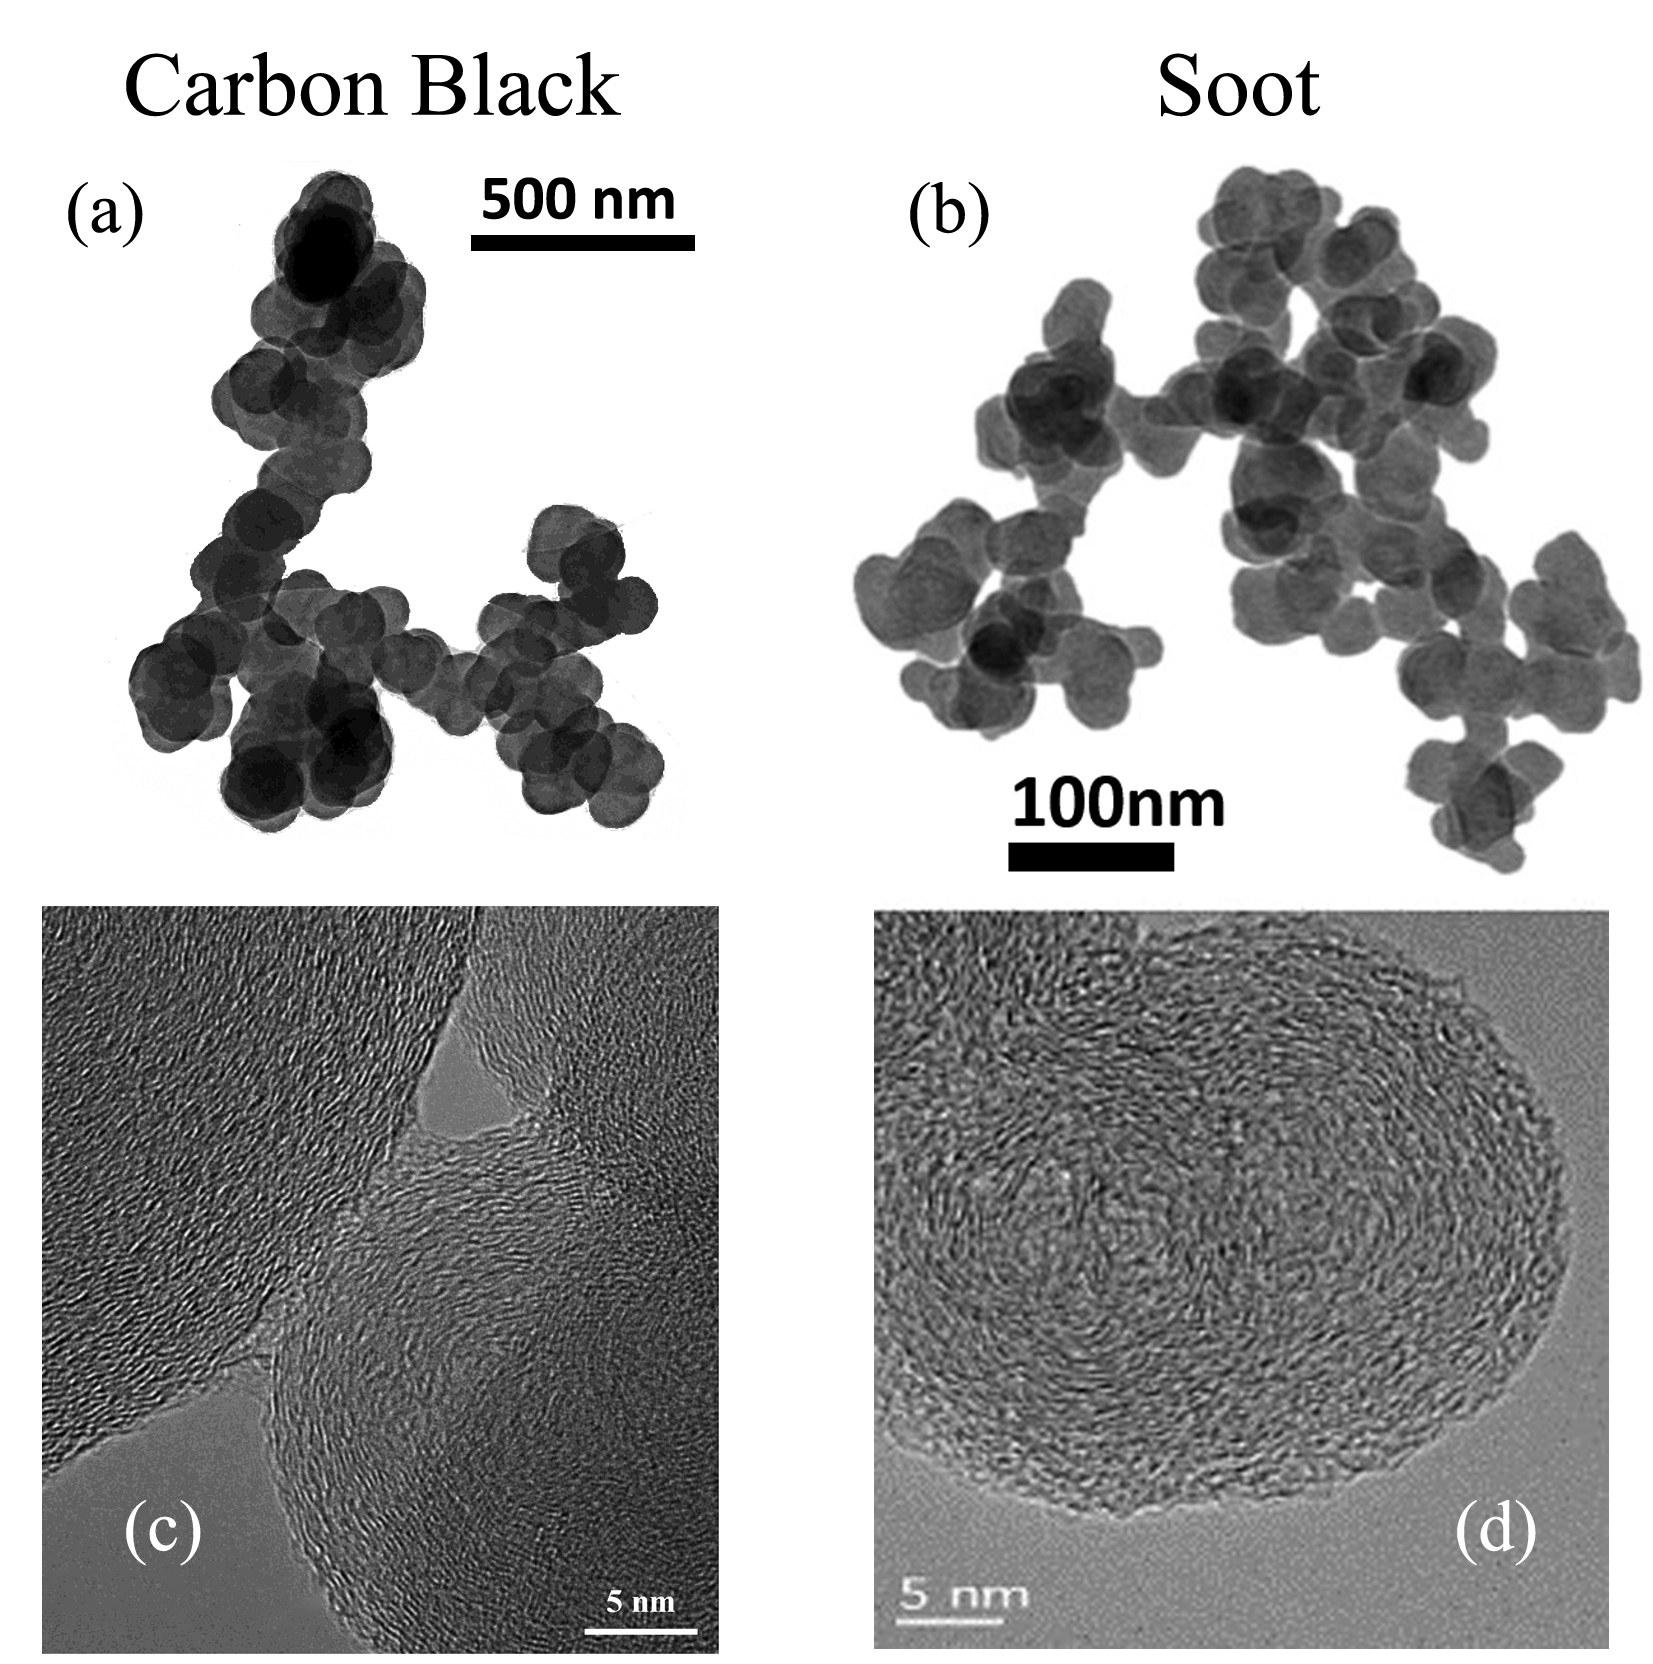
\includegraphics[height=60mm, ]{Figures/Introduction/soot_CB_HRTEM.jpg}
	\caption{The TEM images of Carbon black (a \& c)~\citep{singh2018nanostructure} and soot (b \& d)~\citep{vander2007hrtem, lapuerta2017morphological}
	\label{fig:sootCBHRTEM} that shows soot and CB has similar morphology and structure}
\end{figure} 



\section{Background}
\subsection{Soot inception and surface growth}
Soot formation is a complex process which involves gas phase chemistry, gas-to-solid transition, heterogeneous reactions on solid particles, and aerosol dynamics~\citep{d2009combustion}. It starts with inception which refers to the birth of \textit{"incipient"} soot particles. The elementary reactions leading to soot inception are still elusive due to coupling with gas chemistry~\cite{Wang2011}, dependence on local temperature~\citep{gleason2018effect} and pressure~\cite{gleason2021pahs}. It has also been challenging to pinpoint the start of inception because of its short time scales in the order $10^{-9}$ s~\citep{buesser2012design}, the lack of a decisive criterion to distinguish molecules from particles~\citep{d2009combustion}, and the overlap of inception with particle growth and agglomeration~\cite{martin2022soot}. Despite these limitations and challenges, our knowledge about soot formation has significantly increased thanks to advances in diagnostics methods and reaction mechanism development. 

\begin{figure}[!htbp]
	\centering
	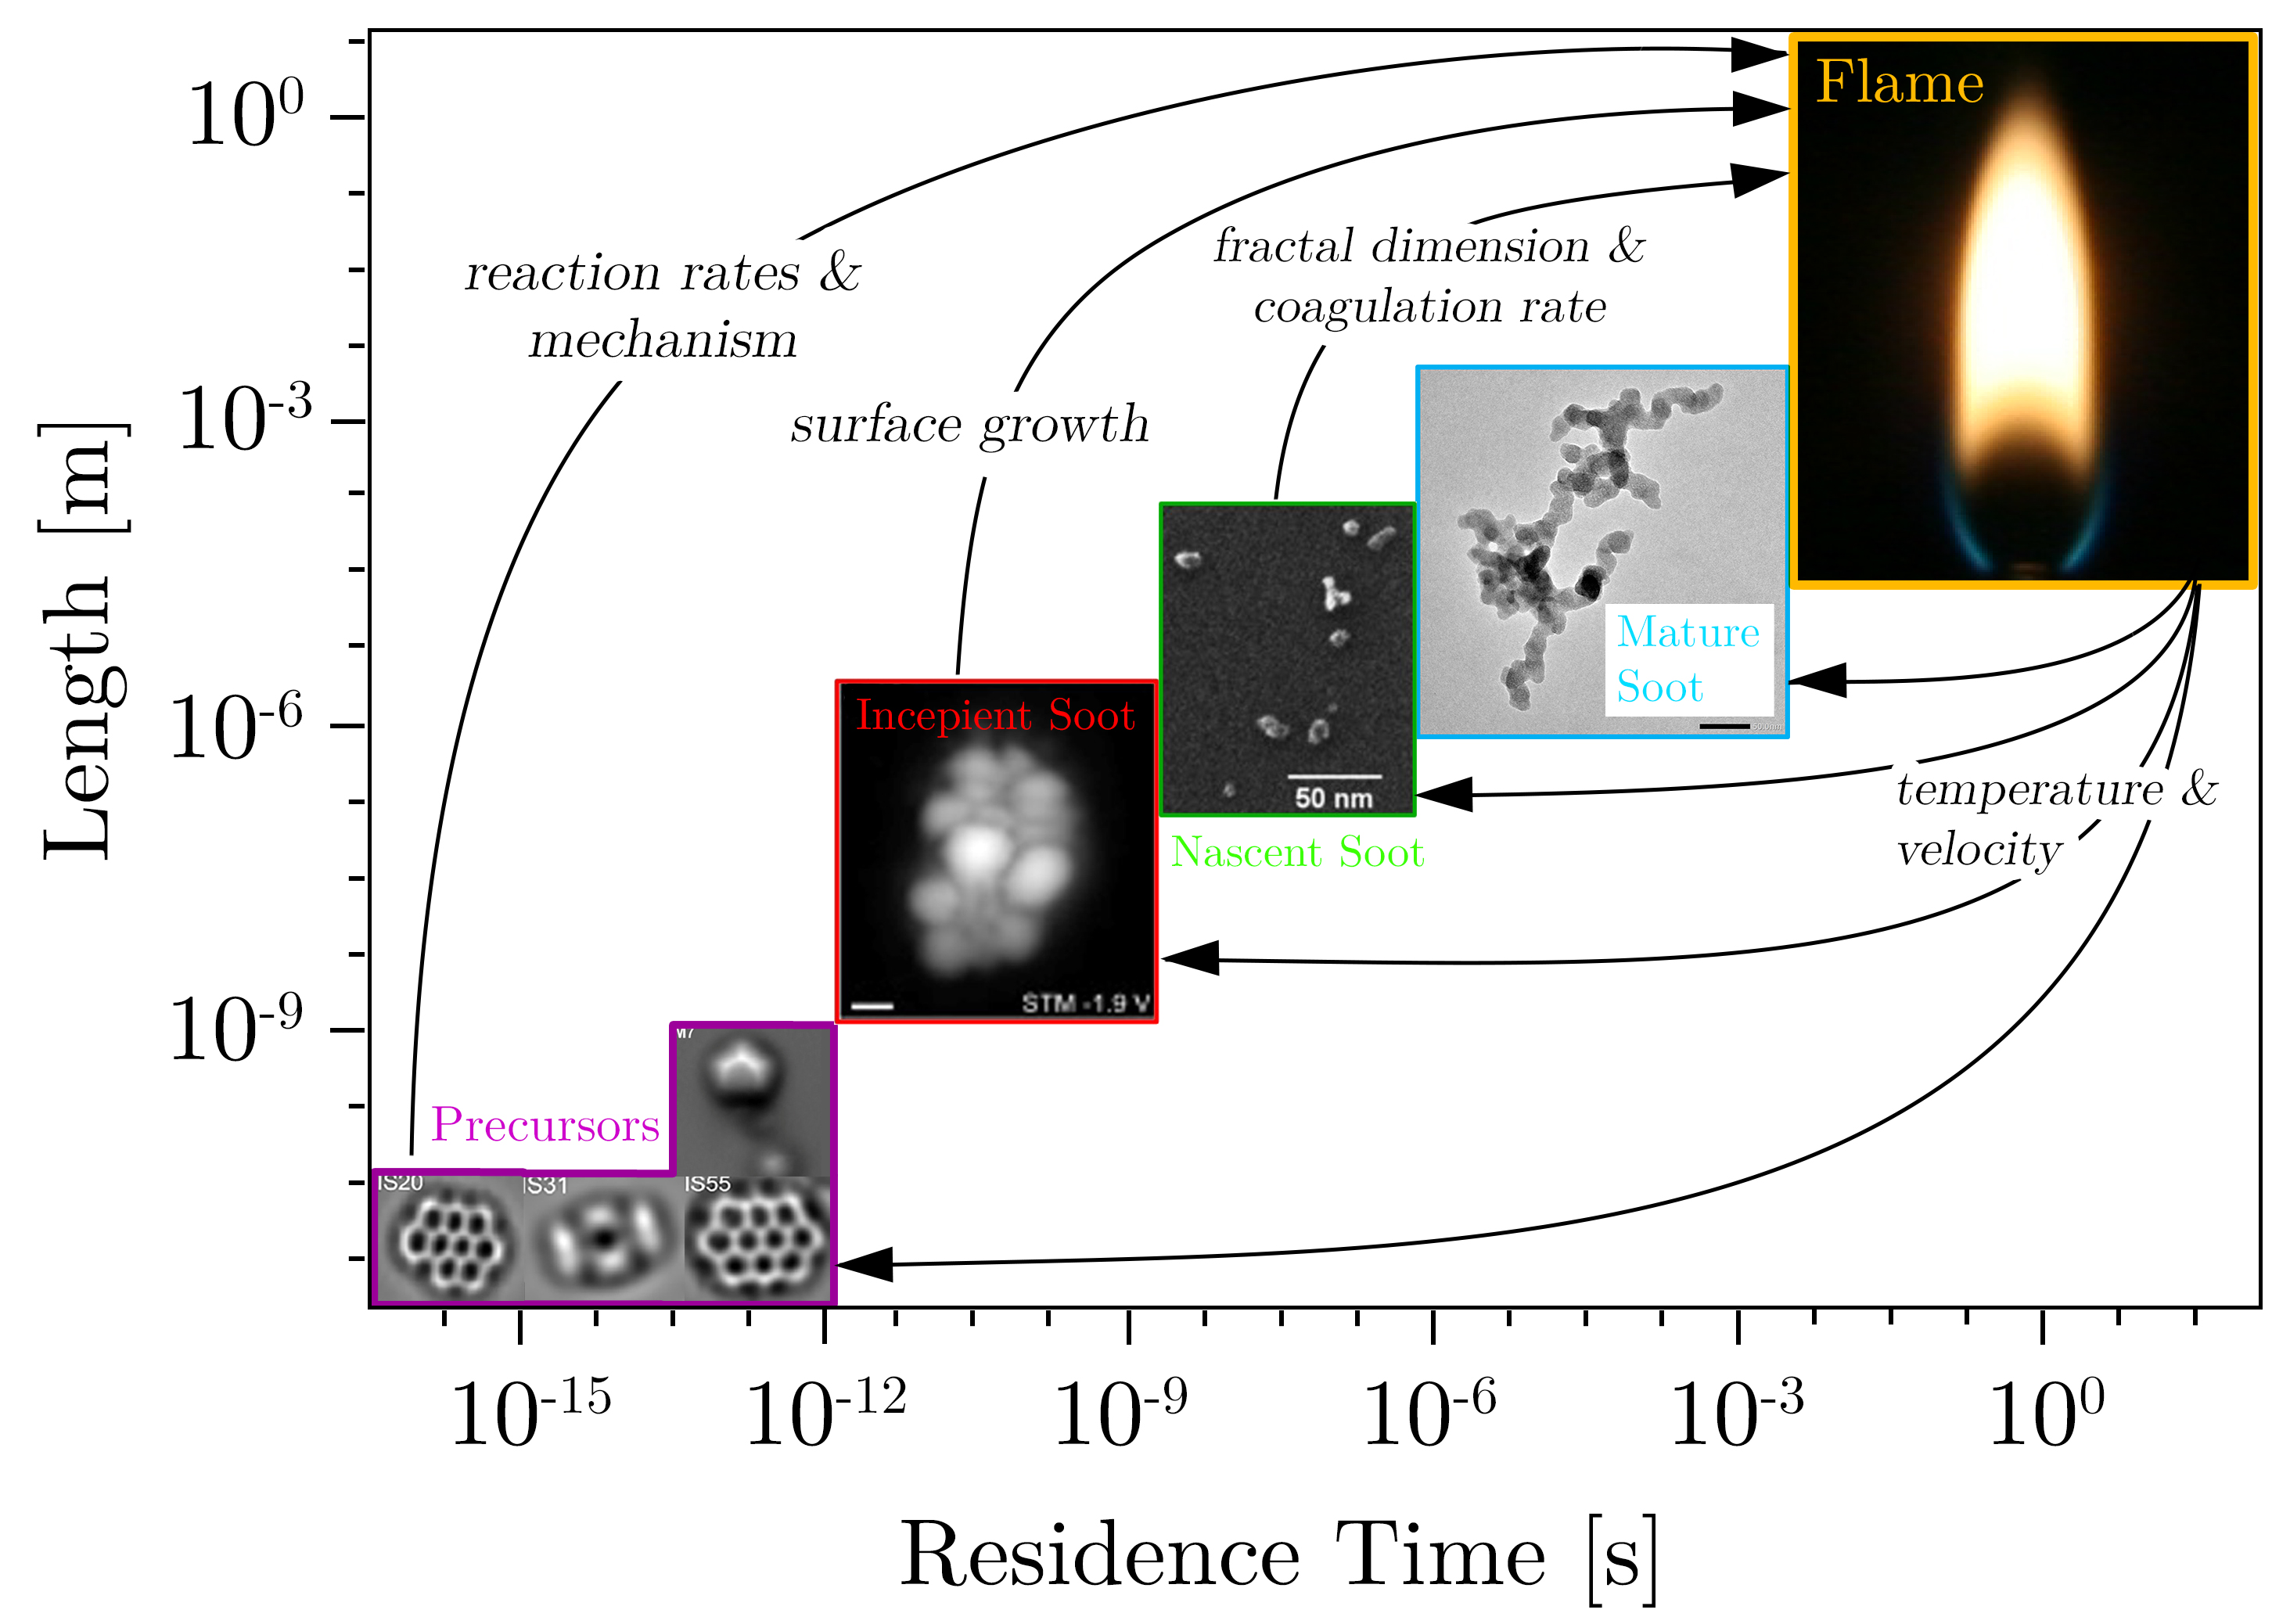
\includegraphics[height=80mm, ]{Figures/Introduction/schematics.jpg}
	\caption{The range of time and length scales of the processes involved in soot formation from molecular reactions to particle-fluid interaction in flames}
\end{figure}

There is compelling evidence that highlights the role of Polycyclic Aromatic Hydrocarbons (PAH) as the main soot precursors. They are thermodynamically stable enough to withstand dissociation at high flame temperatures~\citep{stein1985high} and observed in stacked layers in High Resolution Transmission Electron Microscope (HRTEM) images of soot primary particles~\citep{Oberlin1984}. 

\hl{[placeholder for literature review on the role of diradicals and resonantly stabilized radicals in soot inception]}

But, the two important questions need to be answered: (1) which PAHs contribute most to the inception, and (2) what pathways best describe PAH to incipient soot transition. Purely chemical growth mechanisms are shown to underpredict inception rates and particle size~\citep{frenklach2002reaction}. The bimodality of particle size distribution in premixed flames~\citep{camacho2015mobility} suggests a mechanism second order with respect to the monomer~\citep{Wang2011}. To satisfy these requirements, a collision-based inception was proposed where irreversible polymerization form PAH clusters held together by Van der Wales forces. The theory postulates that PAH growth continues to reach a certain mass threshold that marks emergence of solid particles, but for practical purposes, a dimer is usually considered as incipient soot. 

In this model, hereafter referred to as \textbf{Irreversible Dimerization}, the collision of two PAH molecules is assumed to form a dimer
% that gains mass via two growth mechanisms: (i) hydrogen-abstraction-carbon-addition (HACA) that assumes soot surface to consist of hydrogenated sites with predefined density that can lose hydrogen and react with acetylene (ii) collision of PAH molecules/clusters with soot particles leading to chemisorption. 
Irreversible Dimerization has been used to predict soot formation in burner-stabilized premixed~\citep{salenbauch2015modeling, desgroux2017comparative}, counterflow diffusion flames~\citep{wang2015soot, xu2021experimental}, coflow diffusion flames~\citep{kholghy2016core, veshkini2016understanding}. A collision efficiency factor ranging between $10^{-6}$ to 1 is also employed to adjust the inception flux and PAH adsorption rates to achieve desired soot mass and size distribution. PAHs of moderate sizes such as pyrene (4 rings) to coronene (7 rings) have been considered as the starting point of inception due to their thermodynamic instability that justifies the irreversibility at high temperatures~\citep{frenklach1991detailed}. \citet{blanquart2009analyzing} introduced a two-step However, the theoretical calculations~\citep{miller1985calculations} and experiments~\citep{sabbah2010exploring} indicated that pyrene dimerization is highly reversible in flame condition. 

The inception rate of irreversible dimerization is mainly controlled by PAH concentration due to weak temperature dependency, so it produces new particle in low temperatures (even less than 500 K)~\citep{naseri2022simulating} despite experimental evidence for termination of inception below 1200 K~\citep{sanchez2012polycyclic, cho2016synthesis}. Also, the arbitrary selection of efficiency factors alters the distribution of mass between inception of surface growth the could significantly change soot mass, PSD, and morphology strongly~\citep{saffaripour2014experimental}. \citet{miller1991kinetics} used equilibrium constant for PAH dimerization to calculate the net dimerization rate and demonstrated that the collision of PAHs larger than circumovalene ($\sim$800 amu) could last long enough grow into incipient soot. However, the concentration of PAHs drops rapidly with size~\citep{Wang2011}. The entropy barrier of dimerization is significant for larger PAHs~\citep{giordana2011theoretical}.  


\citet{eaves2015importance} relaxed the irreversibility assumption, and developed a reversible clustering model to simulate inception using an array of PAHs from naphthalene to benzo-pyrene. Building on that work, \citet{kholghy2019role} emphasized on the necessity of chemical bond formation after physical PAH clustering for accurate prediction of volume fraction, primary particle diameter and PSD in ethylene coflow diffusion flames. Later, \citet{kholghy2018reactive} proposed the \textit{"Reactive Dimerization"} model which starts with reversible collision of PAHs leading to physical dimers held with vdW forces that are graphitized and form chemically-bonded dimer that serve as soot nuclei grow via surface reactions. They also performed a systematic analysis on contribution of different PAHs, and concluded that one- and two-ring aromatics account for almost all of inception flux in the so-called \textit{"sooting flame"}~\citep{desgroux2017comparative}. However, \citet{frenklach2020mechanism} pointed out that an inception model that initiated with a highly reversible step similar to Reactive Dimerization~\citep{kholghy2018reactive} cannot produce sufficient flux of particles to match measurements of the benchmark burner-stabilized stagnation flame~\citep{abid2009quantitative}. Instead, they proposed a HACA-driven mechanism where addition of monomer molecule to its radical activated by hydrogen abstraction for a stable dimer via an E-Bridge bond formation, and this sequential process continues to form trimers, tetramers, and larger PAH clusters.

After inception, soot particles grow by the addition of small hydrocarbon species to their surface. This process is described by
the famous hydrogen–abstraction–acetylene–addition (HACA)
mechanism~\citep{frenklach1991detailed, appel2000kinetic}  that assumes the soot surface to consist of hydrogenated sites with a predefined density. Mass growth on soot surface requires H-abstraction to form a radical
site, followed by acetylene attack similar to growth of PAH molecules in the gas-phase. The reactivity of these sites depends on with time and temperature~\citep{woods1991soot, dasch1985decay}. However, soot mass growth without the presence of H radicals~\citep{singh2006numerical} indicated the incompleteness of the HACA mechanism to
describe the entire process of soot surface growth.

Adsorption of PAHs on the surface of soot particles is also a viable growth mechanism~\citep{frenklach1991detailed}, more specifically called physiorption or chemisorption depending on the mechanisms driving the adsorption process~\citep{michelsen2020review}. There is still debate over the stability of adsorbed PAH molecules on soot surface~\citep{obolensky2007interplay}. Following the hypothesis that PAHs are building blocks of soot particles, a mechanism similar to inception is often used to describe  PAH-soot growth.

In typical soot formation processes such as flames and reactor, soot particles are formed at high concentrations (~$10^{12} \#/cm^3$), and inception and surface growth are relatively short compared to the total residence of soot particles. As a result, coagulation becomes dominant rapidly attaining both~\citep{Goudeli2016}
self-preserving size distribution (SPSD)~\citep{lai1972self} and asymptotic fractal-like structure~\citep{mountain1986simulation}.
The evolving fractal-like structure of agglomerates quantified by their mobility diameter normalized by primary particle, $d_m$⁄$d_p$, and gyration, $d_m$⁄$d_g$, diameters can be described with power laws derived from mesoscale simulations~\citep{Kelesidis2017}. The collision frequency of agglomerates depends on their evolving fractal-like morphology. Also, polydisperse agglomerates collide more frequently than monodisperse ones. The enhancement in their collision frequency reaches an asymptotic value of 35\%~\citep{Goudeli2016} or 82\%~\citep{kelesidis2021self} in the free molecular or transition regimes, respectively at SPSD regardless of the polydispersity in their constituent primary particles. Particle morphology formed by inception, surface growth and agglomeration can be tracked precisely by mesoscale simulations, such as Discrete Element Modeling (DEM)~\citep{Kelesidis2017Flame}. However, they are computationally expensive and interfacing them with chemical kinetics in computational fluid dynamics (CFD) simulations is not trivial~\citep{kelesidis2021perspective}. This limits their application. So, sectional population balance models (SPBM) are often used to track agglomerate and primary particle size distribution~\citep{Xiong1993}, morphology~\citep{park2005aerosol}, and composition~\citep{kholghy2016core} in complex laminar~\citep{kholghy2016core} and turbulent flows~\citep{schiener2019transported}. Using the SPBMs coupled with relations for agglomerate fractal-like structure~\citep{matsoukas1991dynamics} and collision frequency [36], particle size distribution, morphology and composition can be tracked accurately. However, the computational cost of SPBMs increases exponentially with the number of sections [31] and particle properties~\citep{kholghy2016core} tracked. Thus, one property (e.g. agglomerate mass) is typically tracked with SPBMs to reduce computational cost. This does not allow to account for agglomerate fractal-like structure~\citep{smooke2005soot, aubagnac2018soot} which limits SPBM accuracy in predicting surface growth and coagulation rate of agglomerates and their size distribution.

Alternatively, particle dynamics can be tracked by the method of moments (MOM)~\citep{kazakov1998dynamic} or monodisperse population balance models (MPBM)~\citep{kruis1993simple}. Such models only track average particle properties (e.g. moment ratios) and their accuracy could be limited if unrealistic assumptions (e.g. approximating agglomerates as monodisperse and perfect spheres) are used. However, when inception and surface growth are short~\citep{Spicer2002} and high particle (number) concentrations are formed~\cite{Kelesidis2017}, they lead to rapid attainment of self-preserving size distributions (SPSD) and agglomerates having asymptotic structure~\citep{Goudeli2016}. In this case a MPBM or MOM can be assembled on a firm scientific basis with accuracy on par with DEM~\citep{Kelesidis2017Flame}, SPBM~\citep{kelesidis2019estimating} and experimental data ~\citep{abid2008evolution, ma2013soot, camacho2015mobility}. Such models can be readily interfaced with CFD simulations~\citep{grohn2012fluid} without significant computational cost, making them ideal for three-dimensional and even turbulent flame simulations. 

The MOM tracks moments of the PSD and estimates average particle properties such as mass~\citep{pratsinis1988simultaneous}, surface area~\citep{blanquart2009joint}, the number of constituent primary particles per agglomerate, $\mathrm{n_p}$~\citep{kazakov1998dynamic}, or even particle compositio~\citep{blanquart2009analyzing} using the ratio of the moments. The MOM with four equations was used to describe synthesis of optical fibers by simultaneous reaction, diffusion, coagulation and thermophoresis of $\mathrm{SiO_2}$ in laminar flow reactors assuming a lognormal PSD~\citep{kim1988manufacture}. The MOM with interpolative closure (MOMIC) was developed to predict simultaneous nucleation, surface growth and coagulation of soot agglomerates and estimate its PSD with six equations~\citep{kazakov1998dynamic}. To calculate source terms of the transported moments, additional moments that are not tracked are needed preventing the closure of the system of differential equations with the MOM~\citep{pratsinis1988simultaneous, frenklach1987aerosol}. Thus, often the PSD shape is assumed a priori~\citep{pratsinis1988simultaneous} or extra equations are solved to estimate it~\citep{kruis1993simple}.

The MPBMs do not have the closure problem and calculate average particle properties by tracking their total concentration, mass \citep{kruis1993simple} and area~\citep{tsantilis2004soft, lindstedt1994simplified}. \citet{kruis1993simple} used a 2-equation MPBM (known as the semi-empirical model) to track soot concentration and mass in (non-premixed) flames assuming spherical particles. Good agreement was achieved for measured soot mass. However, the specific surface area~\citep{lindstedt1994simplified} and coagulation frequency of spheres are significantly smaller compared to that of agglomerates with the same mass underestimating their oxidation rate~\citep{kelesidis2019estimating} and overestimating their concentration [40]. \citet{kruis1993simple} proposed a 3-equation MPBM to account for the fractal-like structure of nanoparticle agglomerates during coagulation and sintering. Agglomerate volume and area were used to obtain their equivalent primary particle diameter, $\mathrm{d_p}$, and $\mathrm{n_p}$. Then, agglomerate collision diameter, i.e. $\mathrm{d_g}$, was calculated by $\mathrm{D_f}$, $\mathrm{d_p}$ and $\mathrm{n_p}$ to account for their fractal-like structure that affects their collision frequency. \citet{tsantilis2004soft} extended the MPBM to predict hard-(chemically-bonded) and soft- (physically-bonded) agglomerates during synthesis of $\mathrm{SiO_2}$ and $\mathrm{TiO_2}$~\citep{grass2006design} nanoparticles with simultaneous reaction, surface growth, coagulation and sintering. Such a MPBM applies best at high concentrations when inception and surface growth are short~\citep{Spicer2002} resulting in the dominance of coagulation where particles rapidly reach their SPSD and asymptotic fractal-like structure. This is often the case for soot emitted from a variety of combustion devices or CB reactors where inception and surface growth are limited to only a few milliseconds when temperature is very high (i.e. T$\ge$1500K)~\citep{kholghy2018reactive}.


%While, this approach can describe inception in low to moderate temperature (<1000 K), and adjusts the inception flux , but it cannot explain how physically-bonded dimers withstand fragmentation at high flame temperatures (>1000 K).      The initial simple The initial PAH classic dimerization describes the inception by physical collision of PAH molecules that  

% 




